\chapter{Background}
\label{chap:background}

In this chapter the background needed to understand the problem of visual place classification and novelty detection will be presented.
It should be enough to introduce several concepts to a reader unfamiliar with computer vision and machine learning areas.
And for readers seeking deeper detail all the concepts have been referenced to papers presenting them.

\section{Visual Place Classification}
\label{sec:place-classification}

\begin{figure}[here]
\begin{center}
\includegraphics[width=0.9\textwidth]{place_classification}
%\caption{Place classification deals with the problem of mapping a given location to a set of known concepts}
\end{center}
\end{figure}

Place Classification deals with the problem of mapping a given location to a set of known concepts.
In this thesis work its assumed the existence of labelled data (sample inputs where the correct label is known) that the algorithm can use during a training step, this is known as supervised-learning.
After the learning step the algorithm is feed with new data and is expected to guess the correct label.

It may feel natural then to pose the classification problem as a probability estimation problem of all the classes and pick the most likely. And several algorithms exists to perform that kind of analysis on data.
Though the problem of probability density estimation is harder than the problem of classification as it requires a full estimation over input space instead of a single decision between classes.
And one should not try to solve an harder problem.

So the usage of discriminative solutions, such as Support Vector Machines, is expected to lead to easier solutions.

There exists several methods that can be used for classification problem such as usage of \emph{Neural Networks}, \emph{Nearest-neighbours}, \emph{Decision Trees}, \emph{Bayesian Networks} and other statistical tools for regression and statistical analysis.
Though since only \glspl{SVM} are used on this work only a short overview over them is provided. For extended knowledge in the methods the reader is advised to look on other materials~\citep{bishop2006pattern}.

\subsection{Support Vector Machines}
\Glspl{SVM} where introduced by \cite{cortes1995support} and can be seen as discriminative linear based classifier.
They are based on a strong mathematical foundation and have powerful generalization capabilities.
In their original form \gls{SVM} separates two classes of points in an hyper-space with a \emph{maximal margin hyperplane}~(\autoref{fig:svm-sample}).

Later they were extended to deal with noisy data by using \emph{soft margins}.
And to handle non-linear spaces as seen on \autoref{sec:kernel-trick}.
Although they only allow for two class-classification several methods have been proposed to build multi-class classifiers based on binary classifiers as seen on \autoref{sec:multiclass-classifiers}.

\begin{figure}[h]
\begin{center}
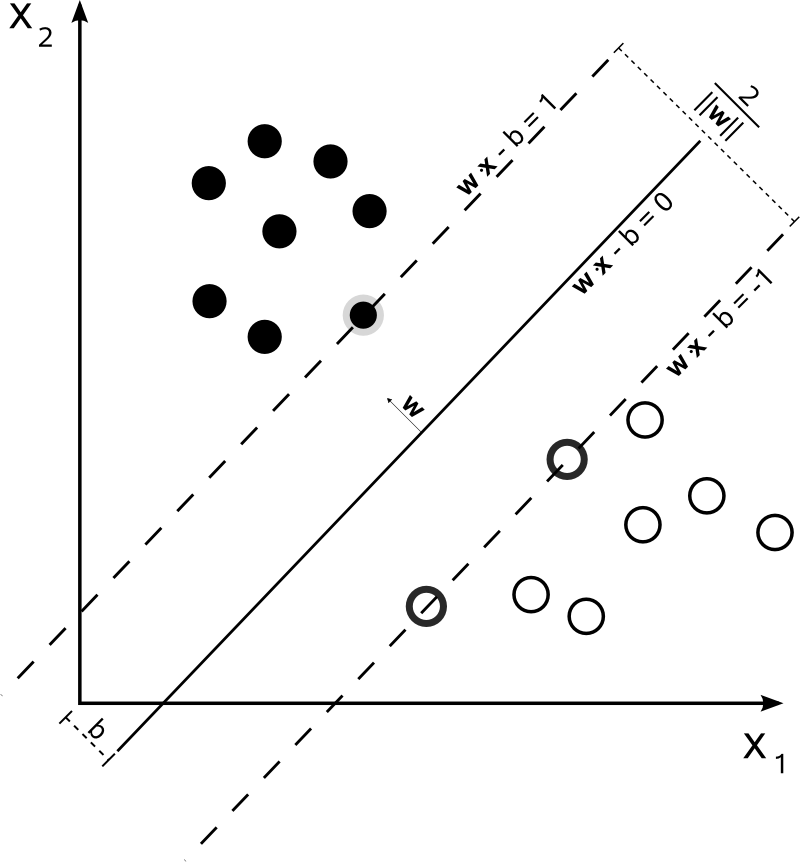
\includegraphics[width=0.5\textwidth]{Svm_max_sep_hyperplane_with_margin}
\end{center}
\caption{{SVM} separating two class of points by a \emph{maximal margin hyperplane}. The hyperplane can be described by the collection of support vectors and associated weights, marked in the image as sample points with large borders.}
\label{fig:svm-sample}
\end{figure}

They have been used in several classification and recognition problems and are in fact a standard across machine learning techniques.
Their efficiency, exact training results and generalization made their suitable for many tasks. Such as text categorization, digit-recognition, spam-classification.
They have also been extensively used in visual place classification~\citep{pronobis2005msc}.

\subsection{The Kernel Trick}
\label{sec:kernel-trick}
\gls{SVM} in their basic form are only able to handle linear spaces.
Nonetheless the classes are most of the time not linearly separable in the input space.
Although there might exists a transformation $\phi$ from the original space into a space $H$ where the input becomes linearly separable.

The Kernel trick allows to extend the \gls{SVM} definition to work on such space $H$ without ever performing an implicit transformation between spaces.
Being enough for that to have a Kernel function defining an inner-product inside such space: $K(x_i, x_j) = \phi(x_i)\cdot\phi(x_j)$.
In that sense a Kernel function can be seen as a function that calculates some similarity measure between two inputs.

Several kernel functions have been proposed being the most commonly used:

\begin{description}
\item[Polynomial Kernel] - $K(x, y) = (x \cdot y + p)^d$
\item[Radial Basis Function] - $K(x, y) = e^{-\gamma\|x - y \|^2}$
\item[Histogram intersection] - $K(x, y) = e^{-\gamma \chi^2(x,y)}$, where $\chi^2(x,y) = \sum_{i=1}^{N}\frac{(x_i-y_i)}{x_i+y_i}$ introduced by \cite{barla2003histogram} allows to compute histogram similarity.
\item[Matching Kernels] - mimic matching similarity and are used when each sample is represented as a set of features~\citep{boughorbel2005intermediate}.
\end{description}

\subsection{Extending to Multi-class}
\label{sec:multiclass-classifiers}
\Glspl{SVM} were designed as two-class classifier. And so they need to be adapted for using in multi-class problems.
The most common usage is to design multi-class classifiers recurring at the usage of multiple two-class classifiers and methods for combining them.
The most typical approaches for a multi-class classification on $c$ classes using \glspl{SVM} are:

\begin{description}
\item[One Against All] - in this method $c$ distinct classifiers are trained to distinguish any class of the remaining ones.
The output of all those classifiers (distance to the separating hyperplane) is then used to categorize the output.
The most common approach is to pick the class with the largest hyperplane distance.
Other variations exists as is the case of using the minimal distance to the average classification distance of each class~\citep{pronobis2007confidence}.

\item[One Against One] - in this method $c*(c-1)/2$ classifiers are trained to distinguish between each pair of classes. The final decision is based on the output of all those classifiers being common to use a majority vote strategy.
\end{description}


\subsection{Features}\label{sec:features}
A feature is a piece of information which is expected to reveal information for solving a specific task.
In that sense features are task-dependant and they will yield different performance based on the type of task they are applied to.

A wanted property on features is its repeatability under similar conditions for the problem in hand. This is: they should be stable and invariant across unwanted types of transformations and noise.
For example a visual feature for object detection should be present even if the target object was translated, scaled, rotated, the light-conditions have changed or even if the object is partially occluded.

Extracting features with those properties allows to greatly reduce the size of input by removing unwanted noise and useless information from the captured data.
Turning the classification problem easier, more reliable and more efficient.

Often several and different types of features need to be extracted. It has been reported by \cite{pronobis2010ijrr} that using multiple features provides a great benefit in the context of place classification.
And \cite{quattoni2009recognizing} has showed that different types have different impact in indoor scene recognition based on the type of scene matching.
Namely was seen that some room-categories are more likely to be recognized by the presence of some objects and others by it generic appearance.

In the context of robotics, sensors such as cameras, laser scans are used to sense the surrounding environment, and features can be extracted from all those. Nonetheless as described in \autoref{sec:visual_motivation} the visual sensor is incredibly rich and most of our features will come from it.

Visual features can be seen as belonging to two categories: \emph{local features} and \emph{global features}.
\emph{Local features} describe fine grain properties of a part of image. For example the existence of specific corner or an edge. \Gls{SIFT} (\autoref{sec:sift}) is an example of such feature and has been proven useful for matching points between images and subsequence extension to object detection.

\emph{Global features} such as \gls{CRFH} (\autoref{sec:crfh}) or {gist}~(\autoref{sec:gist}) try to describe the whole image. Either by statistical analysis of features over all the image or by a structured distribution of textures findable in the image.

\subsubsection{{SIFT} - Scalar Invariant Feature Transform}
\label{sec:sift}\label{sec:local-features}
The detection of interesting points has been studied for several years and is the base of several computer vision problems solution. It allows to perform point matching which can be used in several areas from image stitching, 3D reconstruction, video tracking, object detection, etc\dots

The most used method was presented by \cite{lowe1999object}. And its based on building a feature vector for each image. Each of those features is based on \emph{interesting points} detected by detecting maxima and minima of a difference of Gaussian functions applied in a scale-space.
The scale space is used to provide scale invariant detection. Gaussian functions are used as they are the only way to model a linear scale-space.
Each interesting point is then described by a contained that is rotation invariant.

By seeing an object as a set of features points, index and matching is then performed by a high-dimensional search on a database of know objects. After matching objects can be verified for geometric coherence between features.
\Gls{SVM} classifiers can also be trained to detect objects based on this type of local features by using \emph{Matching kernels} (\autoref{sec:kernel-trick}).

\begin{figure}[h]
    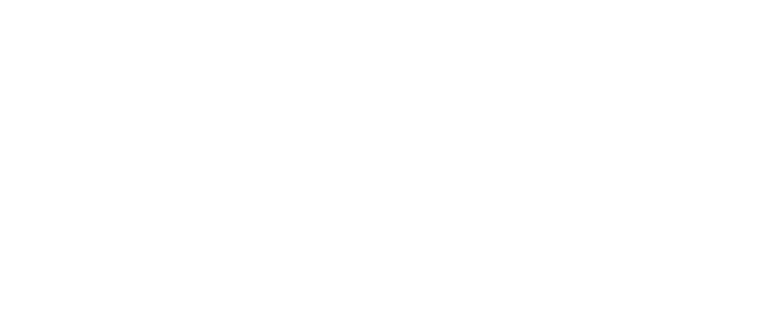
\includegraphics[width=\textwidth]{sift/sift.pdf}
    \caption{{SIFT} and other local features have been proven useful in object detection.}
\end{figure}


\subsubsection{Gist of a Scene}
\label{sec:gist}
\cite{oliva2006building} argue that fast scene recognition does not need to be built on top of object recognition but can be analyzed by scene-centered mechanisms.
They defend that position by pointing out behaviours on human vision:
when provided with a glance of a shot a person can identify the meaning of that given shot or "gist of a scene" without remembering specific details.

\begin{figure}[h]
\center
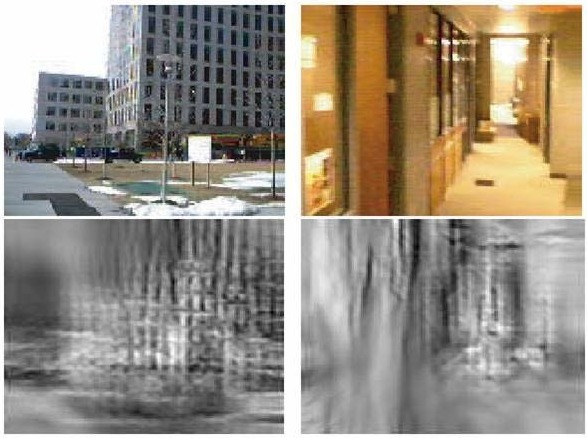
\includegraphics[width=0.60\textwidth]{gist.jpg}
\caption{An illustration of the gist of an image. Top row: original image I; bottom row:
noise image J for which gist(I) = gist(J). We see that the gist captures the dominant
textural features of the overall image, and their coarse spatial layout~\citep{murphy2006object}.}
\end{figure}


\subsubsection{{CRFH} - Composed Receptive Field Histograms}
\label{sec:crfh}\label{sec:global-features}
Composed Receptive Field Histograms are a multidimensional statistical representation of the occurrence of several image descriptors applied to an image.
They can be seen as an high-dimension histogram where each cell records how many pixels of the image have the cell response for the applied descriptors.
Such high-dimensional histogram is expected to be able to better global information contained in the image by capturing several properties of the image as well the relations between them.


\begin{figure}[h]
\begin{center}
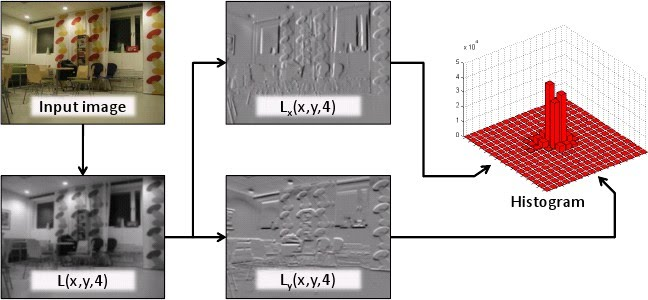
\includegraphics[width=1\textwidth]{crfh_model.jpg}
\end{center}
\caption{A two dimensional histogram of the image built out from two image descriptors: $Lx$ and $Ly$. First-order Gaussian derivatives of image luminance in horizontal and vertical direction applied at a scale 4.}
\end{figure}

Several type of image descriptors can be applied.
For example Gaussian derivatives (such as $L_x$, $L_y$, $L_{xx}$, $L_{yy}$) are partial derivatives of the image luminance after applying a Gaussian filter of a given scale ($\sigma$) on the image.
Gradient magnitude descriptors (such as $|\nabla L|$) can also be used as a rotation invariant descriptor.


One of the problems of high-dimensional histograms is the memory and computationally complexity needed to handle them.
\cite{linde2004object} suggested using a sparse form to represent those by storing only the non-zero-cells in an array structure.

Multidimensional histograms have proven to be useful in the context of object recognition~\citep{schiele1996object}. And have also been previously used in the context of visual place classification~\cite{pronobis2010ijrr}.
\emph{Histogram intersection kernels} (\autoref{sec:kernel-trick}) can be used to train classifiers based on this feature.


\subsection{Other features}
Robots are often equipped with other types of sensors besides cameras and those can be used to extract information from the surrounding environment and yield useful information for the problem of place classification.

An example of such a sensor is a laser scan. Many robots are equipped with them and use it for low-level navigation.
From them its possible to extract a few set of geometric features, such as elongatedness ratios, or room size, which definitely yield important information for place classification.

Currently, with the deploy of the \gls{Kinect} device there has been an increasing usage of depth information available.
We expect that very soon usable features from that type of sensors will be developed.

\begin{figure}[h!]
\center
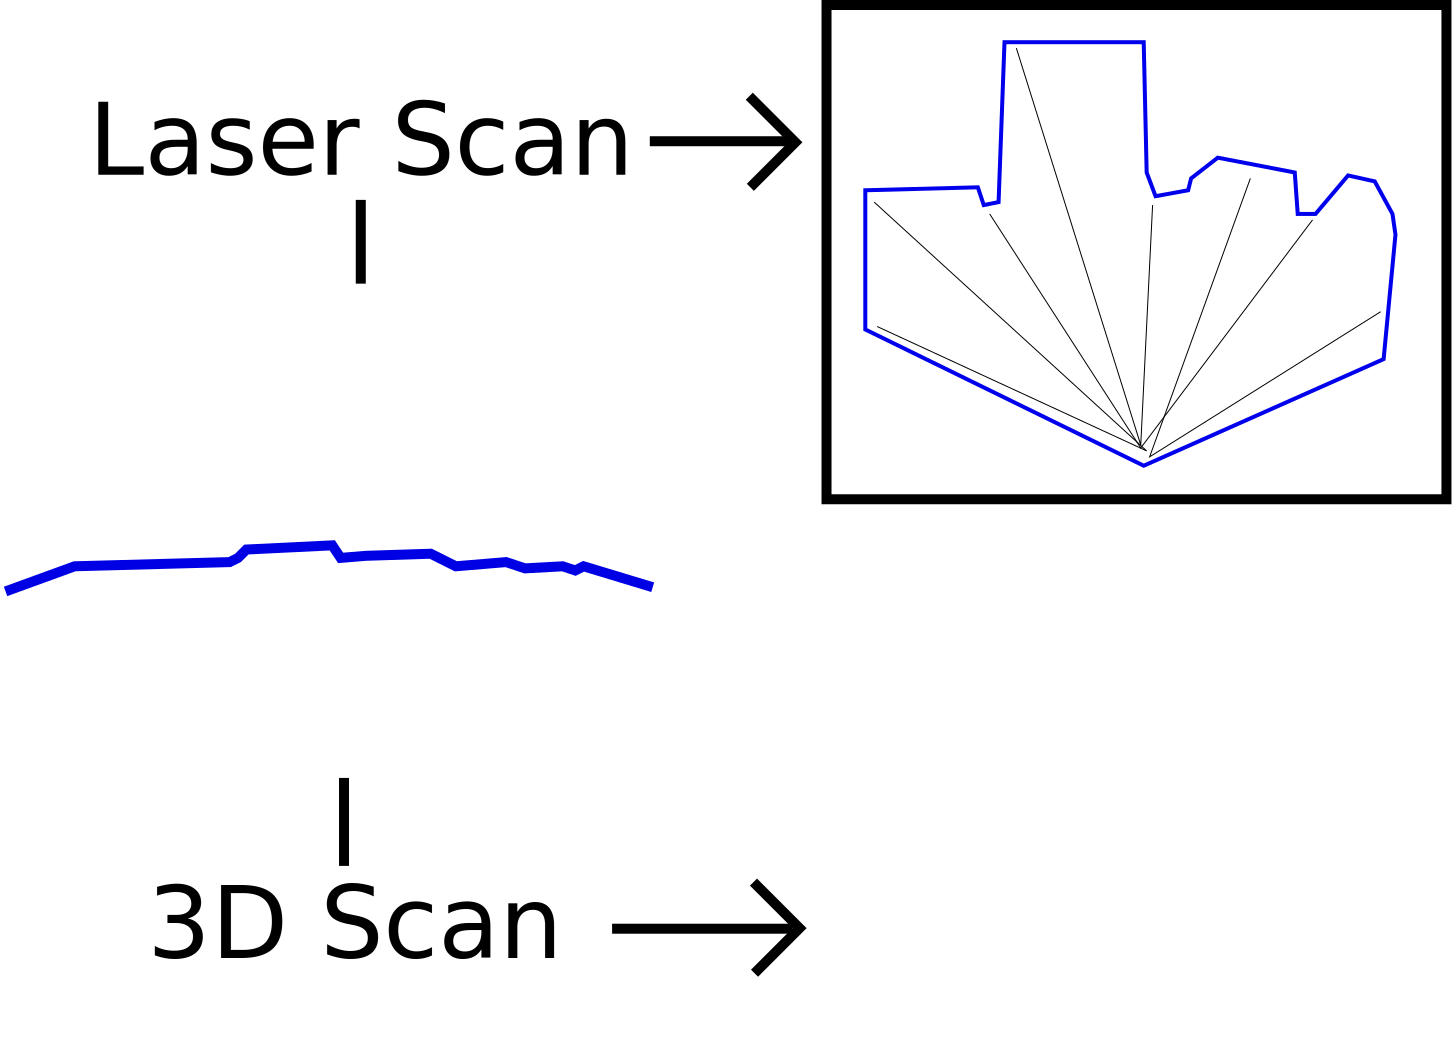
\includegraphics[width=0.5\textwidth]{laser_and_depth_input.pdf}
\caption{Using current laser sensors its possible to extract both 2D and 3D depth information from the environment.}
\end{figure}

\subsection{Spatio-temporal Accumulation}
\label{sec:accumulation}
In the context of robotics, data is not only available as a single-instant (eg.: single frame) but its acquired across time and space as the robot moves through the environment.
This can be used to further improve place classification by accumulating the several clues extracted by the robot for a given position and time.

By using odometry data (such as position and heading) its possible to create a view-point dependent histogram of the robot observations, which can be integrated using discriminative techniques and confidence level estimations. This approach greatly increases the reliability of classification methods as turns the classification more robust against noise or unbalanced data (such as a robot staring at a wall). \cite{pronobis2010ijrr} uses this technique.


\newpage
\section{Novelty Detection}
\label{sec:novelty-detection}
Novelty detection, also called outlier or anomaly detection, is the classification problem related with identification of new or unknown data that the system was not aware of during the training.

It has several applications such as fault detection, intrusion detection, detection of masses in mammograms, hand written digit recognition and many others~\citep{markou2003novelty}.
And has seen an increase of its application in the area of robotics and control.

It is posed as a one class classification where there is only access to the positive samples.
The objective then is to classify new inputs as being generated by the class it was trained or if they belong to some new unknown one.

Either by impossibility of generating samples of "unknown", or by extreme difficulty to acquire negative-examples, two-class classifiers cannot be applied to this problem.
Several other methods were developed to address this problem and they often can be categorized in the following approaches:
based on probability density estimation;
based on using the feature space to separate the given class from others, such as one-class \gls{SVM};
and based on reconstruction-error from a lower-dimension.


\subsection{Density estimation}
One of the simplest approach for novelty detection is pose the problem as a probability density estimation problem and use the expected probability of a given input to trigger the case as novel.

Examples of such approaches are Gaussian Mixtures Models and Parzen-window estimators.
In order to reduce the input size, those approaches often employ dimension-reduction techniques such as \gls{PCA}.

This approach is used in \cite{bishop1994novelty} where \emph{novelty detection} is added to a \emph{neural network} system.
On it the density estimation on the input is calculated using a \emph{Parzen window} over training-data and that value is used as a novelty measure. This way they detect novel data that the their network has not seen before and so the expected output of their system is not reliable.

\subsection{One-class {SVM}}
One-class \gls{SVM} approaches try to distinguish the class by separating the training set from all other points in the input space. They try to archive that by enclosing the training set by some structure (example: hyper-sphere)~\citep{scholkopf2000support}.
This leads to a decision boundary and follows the same principal as Vapnik solving classification with \gls{SVM}: do not solve something harder.

\subsection{Reconstruction Error}
Error reconstruction methods for novelty detection use the assumption that the class to be defined lies on a manifold embedded on the input space of higher dimensions.
By using dimensional reduction techniques, they try to defined that manifold and calculate how far a new input is from it.

\label{sec:kernel-pca}
One of the most common methods used for that is \gls{K-PCA}~\citep{scholkopf1997kernel}, which uses the kernel-trick (\autoref{sec:kernel-trick}) to extend \gls{PCA} and perform a nonlinear dimensionality reduction on the input. This technique has been successfully used in novelty detection by \cite{Hoffmann2007863}.

\begin{figure}
\center
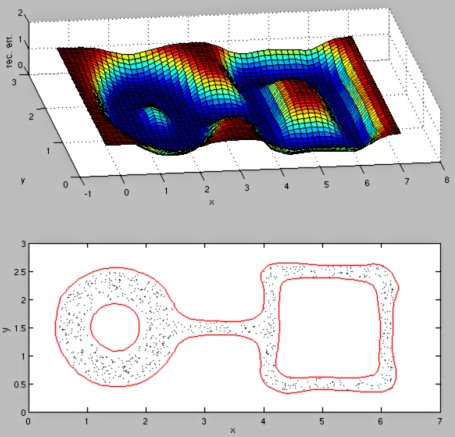
\includegraphics[width=0.50\textwidth]{ringlinesquare_kpca}
\caption{{Kernel PCA} used on a ring-square-circle distribution~\citep{Hoffmann2007863}.}
\end{figure}

\section{Graphical Models}
\label{sec:graphical-models}
Graphical models usage can be tracked back to earlies 1920 but they only become popular in mid-eighties when researchers started to use \emph{Bayesian Networks} to model expert systems~\citep{borgelt2002graphical}.

They serve as a better tool to model \emph{random variables} (nodes on the graph) and their probabilities as they model the conditional dependence between variables (edges on the graph).
Important to note that here \emph{random variables} does not denotes a truly random variable but one that is unknown by the system and is conditioned by other variables/evidences.

This type of graphs provide a generative model where the probability of any given scenario can be determined. As opposed to non-generative models where a given probability can only be calculated if certain data is given.
This means when a graphical model is learned, it can be used to generate new samples from the learned distribution.

They have been successfully used in several machine-learning task such as: information extraction, speech recognition, computer vision. They are also useful due to their ability to deal with semantic (high-level) features~\citep{boutell2006factor} and ability to represent properties of the reality they try to model.

Two main types of graphical models have been used: Bayesian Networks which model directed edges between variables and Markov Random Fields where variables are connected by a potential but no special direction is given to edges.

An important property of these graphs is the \emph{Markov-blanket} of a node.
For a given variable $a$, a \emph{Markov-blanket} is a set of variables in the surroundings of $a$ that when given the value of $a$ becomes independent of the rest of the graph~\citep{pearl1988probabilistic}.
On non-directional graphs it is directly determined by the nodes connected to $a$.
This allows the usage of graph algorithms such as \emph{min-cut} to quickly determine most likely scenarios.
In the case of directed edges a node blanket is also influenced by the direction of the edges and a more complex schemes need to be used.

As \cite{lauritzen2002chain} points this two types of models can be represented as a \emph{chain graph} where both directed and undirected edges can co-exist.
Though this generalization is hard to implement due to mis-understandings on the concepts the graph-models use.

Another useful interpretation of graphical-models are \emph{factor graphs}. Those are able to handle both \emph{Bayesian Networks} and \emph{Markov Random Fields}. Under this interpretation a graph is seen as a bipartite graph that connects variables with factors that influence them~\citep{bishop2006pattern}.
This gives a very useful framework to develop belief propagation on them by seeing a message-passing mechanism between nodes. Belief propagation is used to calculate marginal-probabilities.

\begin{figure}[ht]
    \begin{minipage}[b]{0.3\linewidth}
        \centering
        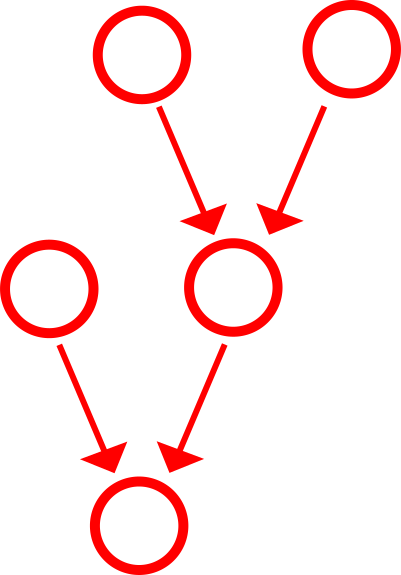
\includegraphics[width=0.8\textwidth]{graphical-models/BayesNet.pdf}
        \caption{Bayes Networks}
    \end{minipage}
    \hspace{0.5cm}
    \begin{minipage}[b]{0.3\linewidth}
        \centering
        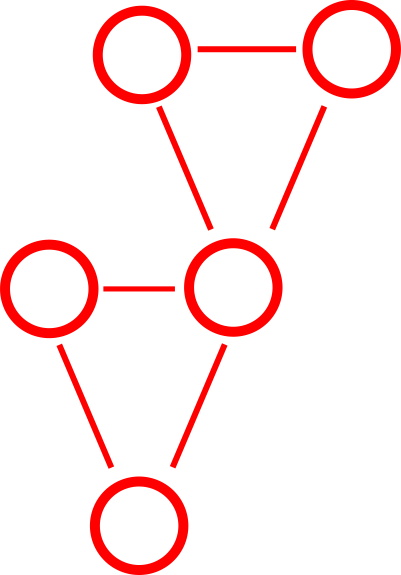
\includegraphics[width=0.8\textwidth]{graphical-models/MarkovRandomField.pdf}
        \caption{Markov Random Field}
    \end{minipage}
    \hspace{0.5cm}
    \begin{minipage}[b]{0.3\linewidth}
        \centering
        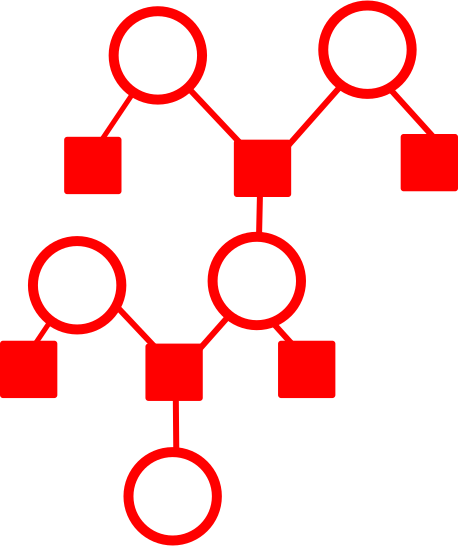
\includegraphics[width=\textwidth]{graphical-models/FactorGraph.pdf}
        \caption{Factor Graph}
    \end{minipage}
\end{figure}
